\Author{\daAuthorOne}

Mobile field teams need address databases that stay up-to-date in real time. However, traditional methods cannot keep up with fast changes, like road closures, new buildings, or street name changes. Manual updates take time, and fixed validation rules do not account for regional differences or typos. These issues can lead to wasted time or even serious risks in critical situations.\blankLine

This chapter explains how adaptive algorithms and real-time data integration can help solve these problems. Adaptive algorithms improve address databases by learning from new data, while real-time systems process live updates instantly. Together, they help mobile apps keep up with changing environments.


    \subsection{Traditional Methods for Address Database Management}

    Traditional address database management relies on manual or semi-automated processes that lack real-time adaptability. These methods were designed for stable environments with occasional data changes, which makes them less effective for modern mobile applications requiring constant updates. This chapter outlines common challenges faced by traditional systems and their limitations.


        \subsubsection{Manual Entry and Batch Updates}
        In the past, address databases were updated through periodic batch uploads, such as monthly CSV files, which store data in a table format with each value separated by commas. Organizations often relied on printed address lists given to field teams, with corrections submitted on paper. This method caused delays. For example, if a street name changed due to construction, mobile teams could work with outdated data for extended periods. \autocite{FasterCapital2025Mar}\blankLine


        Manual data entry by administrators was another common practice. Human errors, such as typos, worsen the problem, making the system less reliable. A study conducted by the Journal of Accountancy found that human error rates in manual data entry can range from 1\% to 5\%. \autocite{integrationmadeeasy2025Mar}

        \subsubsection{Static Validation Rules}
        Address database management systems often rely on strict validation rules, such as regular expressions, to verify address formats. Regular expressions define patterns for strings, making them useful for enforcing specific formats. For example, a regex pattern might require the full word "Street" instead of abbreviations like "St." or "Str.". \autocite{AutorenderWikimedia-Projekte2002Jul}\blankLine


        %bild einfügen
        \begin{figure}[H]
            \centering
            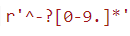
\includegraphics[width=0.2\textwidth]{images/AdminPanel/regexInputFormatter.png}
            \caption{Regular Expression Example}
            \label{fig:regex}
        \end{figure}



        \subsubsection{Third-Party Data Purchasing}
        Third-party data purchasing involves obtaining address datasets from external providers to update and maintain address information. These datasets are usually updated on a regular schedule and cover a wide area. However, the data can quickly become outdated, especially in areas where changes occur rapidly.\blankLine

        Temporary road closures or infrastructure damage might not be reflected in these datasets if updates are infrequent. As a result, teams relying on outdated maps may encounter roads that are blocked or no longer accessible. This lack of real-time updates can cause delays in reaching critical locations or reduce the efficiency of field teams.


    \subsection{Adaptive Algorithms}
    Adaptive algorithms are methods that continuously adjust their parameters in response to new data and changing environmental conditions. These techniques are vital for applications where real-time adaptation is necessary. The following sections describe several core approaches within this domain. \autocite{AdaptiveWikimediaprojects2024Aug}\newpage


        \subsubsection{Fuzzy Matching}
        Fuzzy Matching, also known as Approximate String-Matching or Fuzzy Logic Name Matching, is a string-matching algorithm that helps identify duplicate strings, words, or entries that closely resemble each other, even when there are abbreviations or misspellings. The technique works by applying edit operations such as insertion, deletion, substitution, and transposition to adjust the strings. These operations are measured in terms of an "editing distance," which influences the match score.\blankLine
        
        Fuzzy matching is widely applied in various fields, such as document data extraction, spell-checking suggestions, deduplication, and even genome sequencing. It helps achieve high data accuracy by identifying and matching errors. \autocite{Nieters2024Dec}

        \begin{figure}[H]
            \centering
            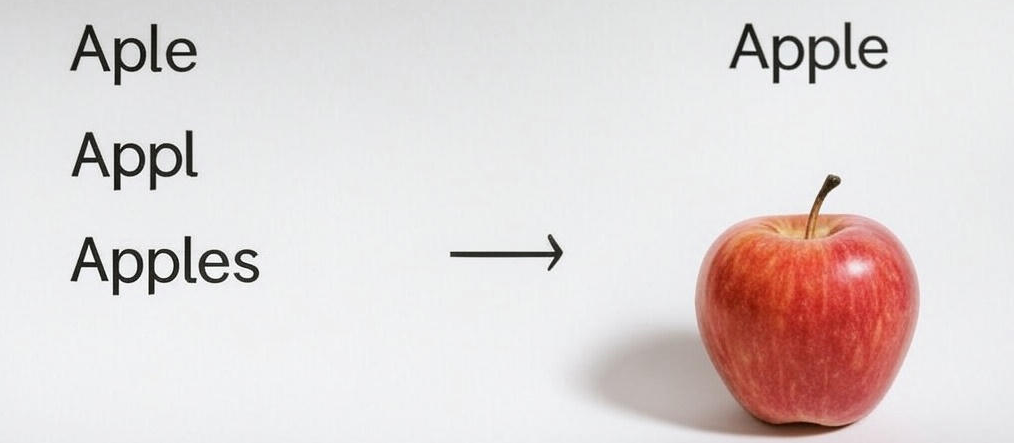
\includegraphics[width=0.5\textwidth]{images/AdminPanel/FuzzyMatching.png}
            \caption{Fuzzy Matching Example}
            \label{fig:fuzzy-matching}
        \end{figure}
        \todo{Quelle von Chat GPT?}

        \subsubsection{Machine Learning Model}
        Machine learning models can be trained to identify patterns in incoming data and update the database dynamically, eliminating the need for manual intervention. These models are particularly effective in rapidly changing environments, as they continuously learn from new data and provide insights to refine address information in real time.\blankLine

        For example, an ML model can detect and predict changes in street names, new construction sites, or temporary roadblocks based on GPS data, social media updates, or traffic reports. By integrating these data streams, the model can anticipate issues not yet reflected in official datasets and make real-time adjustments to the address database. Moreover, as new information becomes available, the machine learning model continuously improves its predictions, adapting to evolving patterns and ensuring the database remains accurate and up-to-date. \autocite{Encora2023Nov}
        
        
        \subsubsection{Rule-Based Filters}
        \label{sssec:rule-based-filters}
        
        Rule-based filters enforce logical constraints on address data to maintain quality and relevance in dynamic environments. A filter could flag addresses lacking GPS coordinates during emergency responses, enforcing manual verification before navigation.\blankLine
        
        
        \textbf{Structure of Rule-Based Filters}\blankLine
        A rule-based filter consists of logical conditions applied to address attributes:
        \begin{itemize}
            \item \textbf{AND}: All rules must be true.
            \item \textbf{OR}: At least one rule must be true.
        \end{itemize}
        

        \textbf{Types of Rule-Based Filters}
        \begin{itemize}
            \item \textbf{Threshold-Based Rules}: Automatically reject addresses with missing or implausible values.
            \item \textbf{Geospatial Rules}: Flag addresses that fall outside predefined operational zones.
            \item \textbf{Historical Consistency Checks}: Detect frequently modified addresses and prompt for manual review.
        \end{itemize}
        
        \textbf{Integration with Adaptive Algorithms}\blankLine
        While rule-based filters provide a structured approach to data validation, they can be enhanced with adaptive algorithms. Machine learning models can analyze user corrections over time and adjust rules dynamically. For instance, if multiple users correct the same address format, the system can learn from these patterns and refine its filtering criteria automatically.
        

    \subsection{Real-Time Data Integration Frameworks}
    Real-time data integration frameworks are systems designed to collect, process, and deliver data instantly as it is generated. Unlike traditional batch processing, which handles data in chunks, these frameworks enable continuous updates. This makes them ideal for applications where delays are unacceptable.

        \subsubsection{Challenges}
        Real-time data integration faces several challenges, particularly in dynamic environments such as mobile field operations: \autocite{vexdata2024Jun}
        
        \begin{itemize}
            \item \textbf{Data Quality:} Errors such as typos or GPS drift require adaptive algorithms for correction.
        
            \item \textbf{Scalability:} Systems must handle thousands of users and sudden data spikes, especially during disasters or high-demand situations.
        
            \item \textbf{Fault Tolerance:} Data loss due to network failures must be prevented.
        
            \item \textbf{Consistency:} Conflicting address data from multiple sources needs resolution.
        \end{itemize}
                
        \subsubsection{Core Components}

        A robust real-time data integration framework consists of four key components: \autocite{Limited2025Mar}

    \begin{itemize}
        \item \textbf{Data Sources:} These include GPS sensors, external databases, and other input streams.  

        \item \textbf{Data Ingestion:} Tools and frameworks collect and efficiently route data streams.  

        \item \textbf{Data Processing:} Engines process, clean, analyze, and enhance the data.  

        \item \textbf{Storage \& Delivery:} Processed data is stored in databases and accessed via APIs.

    \end{itemize}

        \subsubsection{Popular Frameworks}

        Three frameworks dominate real-time integration: \blankLine
        \textbf{Apache Kafka}: A high-throughput streaming platform. It could process GPS and traffic data to reroute teams around road closures.\blankLine
        \textbf{Apache Flink}: A low-latency engine for complex workflows. Flink could power ML models predicting address changes.\blankLine
        \textbf{AWS Kinesis}: A cloud-native service for scalability. Kinesis merges regional address updates into a global view for international teams.\blankLine
        
        Choosing between them depends on needs: Kafka for volume, Flink for processing, Kinesis for cloud scalability. \autocite{Ranjbary2024Sep}


        \subsubsection{Evaluation Metrics}
        \label{sec:evaluation-metrics}

        To assess the effectiveness of adaptive algorithms and real-time data integration, two critical metrics are analyzed: accuracy and latency.

        \paragraph{Accuracy}
        \label{par:accuracy}

        Accuracy measures how closely the addresses in the database match real-world locations, ensuring reliable address information. Traditional methods often suffer from decay over time due to manual updates or infrequent batch imports, leading to outdated or incorrect data.  \blankLine

        Inaccurate data can lead to inefficiencies, delays, or even costly mistakes. Furthermore, achieving high accuracy often involves continuous updates and validation of data, particularly when using multiple data sources. \autocite{GeeksforGeeks2024Oct}\blankLine

        Accuracy is calculated as:
        \[
        \text{Accuracy} = \frac{\text{Correct Addresses}}{\text{Total Addresses}} \times 100
        \]
    

        \paragraph{Latency}
        \label{par:latency}

        Latency measures the delay between data generation and its availability in the app. For mobile teams, latency above 30 seconds can render updates useless during fast-moving operations. Reducing latency is critical for ensuring timely decision-making and operational efficiency. Key factors influencing latency include: \autocite{GeeksforGeeks2024Oct}

        \begin{itemize} 
            \item \textbf{Data Ingestion Speed}: Fast ingestion ensures data is quickly captured, minimizing delays and speeding up availability.
            \item \textbf{Edge Processing}: Local data processing speeds up decision-making by filtering data before transmission, reducing network load.
            \item \textbf{Network Bandwidth}: Latency is affected by network bandwidth; poor conditions, like low signal or congestion, increase delays.
            \item \textbf{Data Prioritization}: Algorithms that prioritize critical data reduce perceived latency by processing urgent updates first.

        \end{itemize}

\blankLine

